% thesis.tex
%
% Description  : Chris Biancone's template for an MS Graduate Paper in EE at RIT, 04/2024
%
% Organization :
%	figures/			% Figures related to the top-level
%	prologue.tex		% Prologue (before the main document)
%	glossary.tex		% Acronymns and glossary
%	mybibliography.bib			% Bibliography
%	<chapter>			% Folder for the <chapter> chapter
%		figures/		% Figures for the <chapter> chapter
%		<chapter>.tex	% Document for the <chapter> chapter
%
%%%%%%%%%%%%%%%%%%%%%%%%%%%%%%%%%%%%%%%%%%%%%%%%%%%%%%%%%%
% Document Type
%%%%%%%%%%%%%%%%%%%%%%%%%%%%%%%%%%%%%%%%%%%%%%%%%%%%%%%%%%

\DocumentMetadata{pdfversion=1.7, pdfstandard=A-2u} % archival PDF with unicode

\documentclass[eeeepaper]{ritthesis}  % Use this line for your thesis document
%\documentclass[cmpeproject,cmpeproposal]{ritthesis}  % Add the option "cmpeproposal" when preparing the proposal for your project research
%\documentclass[cmpethesis,cmpeproposal]{ritthesis}  % Add the option "cmpeproposal" when preparing the proposal for your thesis research

%%%%%%%%%%%%%%%%%%%%%%%%%%%%%%%%%%%%%%%%%%%%%%%%%%%%%%%%%%
% Packages
%%%%%%%%%%%%%%%%%%%%%%%%%%%%%%%%%%%%%%%%%%%%%%%%%%%%%%%%%%

% Style
\usepackage[]{fncychap}
\usepackage{setspace}
\usepackage[normalem]{ulem} % Enable normal \ul underline
\usepackage{url}
\urlstyle{same}
\usepackage{chngcntr}
% \usepackage{microtype}
% \UseMicrotypeSet[protrusion]{basicmath} % disable protrusion for tt fonts

% Tables
\usepackage{tabularx,multirow,array,threeparttable}

% Plots & Color
\usepackage[dvipsnames]{xcolor}
\usepackage{colorspace,tcolorbox,colortbl}
\tcbuselibrary{skins}
\usepackage{pgfplots}
\pgfplotsset{compat=newest}
\usepackage[american voltages]{circuitikz}

% Math
\usepackage{mathtools}
\usepackage{amsfonts,amssymb,nicefrac,sympytex}
\usepackage{siunitx}
\sisetup{detect-all=true}   % ensure proper font weight
%\DeclareSIPrefix\micro{\ensuremath{\symup{\mu}}}{-6} % ensure upright mu for micro
\sisetup{per-mode = repeated-symbol}    % ensure "/" inline unit delineator
\sisetup{range-phrase = {\text{~to~}}}  % SI range clarity (NIST 811 Ch7.7)
\DeclareMathSymbol{\varOmega}{\mathalpha}{operators}{"0A}   % upright omega for ohms
\providecommand*{\upOmega}{\varOmega}   % upright Ohms
\DeclareSIUnit{\sq}{\ensuremath{\Box}}    % sheet resistance
\DeclareSIUnit{\Siemens}{S}
\DeclareSIUnit{\torr}{Torr}
\DeclareSIUnit\sig{\ensuremath{\sigma}} % std dev
\DeclareSIUnit\ppm{ppm}

% Used for creating clicking references
\usepackage[type={CC},modifier={by},version={4.0},lang={english},hyperxmp=false]{doclicense}
\usepackage[]{hyperref,datetime2}
\usepackage[noabbrev, capitalise]{cleveref}
\crefname{lstlisting}{Listing}{Listings}

% Figures
\usepackage{graphicx}

% Support for typesetting subcaptions, uncomment if necessary
% \usepackage{subcaption}
% \usepackage{subfigure}

% Typset indexes - Needed for sorting the glossary
%  - xindy: Sorting / indexing of items
\usepackage[xindy]{imakeidx}

% Support for glossaries
%  - nopostdot: Omit dot at the end of each description
%  - nonumberlist: Supress number of items
%  - acronym: Support for acronyms
%  - toc: Add glossary to table of contents
%  - xindy: Sorting / indexing of items
\usepackage[nopostdot,nonumberlist,acronym,toc,xindy]{glossaries}

% Support for displaying pseudo-code
\usepackage{algorithm,algpseudocode,fancyvrb}
\algdef{SE}[VARIABLES]{Variables}{EndVariables}
   {\algorithmicvariables}
   {\algorithmicend\ \algorithmicvariables}
\algnewcommand{\algorithmicvariables}{\textbf{Variables Definition}}

% To generate the dummy text you'll find all over
\usepackage[english]{babel}
\usepackage{blindtext,lipsum}

% Fonts
\ifpdftex
	\usepackage[utf8]{inputenc}
	\usepackage[T1]{fontenc}
	\usepackage[lcgreekalpha,upint]{stix2}
\fi
\ifluatex
	\usepackage{fontspec}
	\usepackage[warnings-off={mathtools-colon,mathtools-overbracket}]{unicode-math}
	\setmainfont{STIXTwoText}[
	Extension		= .otf,
	UprightFont		= *-Medium,
	BoldFont		= *-Bold.otf,
	ItalicFont		= *-MediumItalic.otf,
	BoldItalicFont 	= *-BoldItalic.otf
	]
	\setmonofont{Fira Code}[
	Extension		= .ttf,
	UprightFont 	= *-Regular,
	Numbers 		= SlashedZero,
	StylisticSet	= {2,5,3,9},
	CharacterVariant= {20,26,30},
  	Contextuals=Alternate
	]

\fi
\usepackage{lstfiracode,matlab-prettifier}
\lstset{
  language=C++,
  style=FiraCodeStyle,
  basicstyle=\mlttfamily
}
\definecolor{backcolor}{rgb}{0.93,0.92,0.95}
\definecolor{codegreen}{rgb}{0,0.6,0}
\lstdefinestyle{myStyle}{
	basicstyle=\ttfamily\footnotesize\selectfont\linespread{1},    
	backgroundcolor=\color{backcolor},   
    commentstyle=\color{codegreen},
	captionpos=b,
	columns=flexible,
    breakatwhitespace=false,
    breaklines=true,    
	extendedchars=true,
	frame=ltb,
	framerule=0pt,         
    keepspaces=true,                 
    numbers=left,       
    numbersep=5pt,                  
    showspaces=false,                
    showstringspaces=true,
    showtabs=false,                  
    tabsize=2,
}
\lstset{style=myStyle}

%%%%%%%%%%%%%%%%%%%%%%%%%%%%%%%%%%%%%%%%%%%%%%%%%%%%%%%%%%
% Macros
%%%%%%%%%%%%%%%%%%%%%%%%%%%%%%%%%%%%%%%%%%%%%%%%%%%%%%%%%%

% For custom IEEEtranDOI.bst to work with hyperkinked DOIs
\newcommand*{\doi}{}
\makeatletter
\newcommand{\doi@}[1]{\href{https://doi.org/#1}{#1}}
\DeclareRobustCommand{\doi}{\hyper@normalise\doi@}
\makeatother

% Default header for a table
\newcommand{\tableheader}[1]{\multicolumn{1}{|c|}{\textbf{#1}}}

% Section referencing
\newcommand{\sref}[1]{Section~\ref{#1}}

% Figure referencing
\newcommand{\fig}[1]{Figure~\ref{#1}}

% Equation referencing
\newcommand{\eq}[1]{(\ref{#1})}

% Algorithm referencing
\newcommand{\alg}[1]{Algorithm~\ref{#1}}

% Glossary referencing
\newcommand{\glsref}[1]{\\ \textit{Glossary:} \gls{#1}}

% Change comment style to use #
\algrenewcommand{\algorithmiccomment}[1]{\# #1}

% Make *proper* vector arrows - Credit to harpoon pacakge for initial idea
\newlength{\argwd}
\newlength{\arght}
\newcommand{\overharp}[3]{%
	\settowidth{\argwd}{#2}%
	\settoheight{\arght}{#2}%
	\addtolength{\argwd}{.1\argwd}%
	\raisebox{\arght}{%
		\makebox[.04\argwd][l]{%
			\resizebox{\argwd}{#3\arght}{\(#1\)}%
		}%
	}%
	#2%
}
\newcommand{\overrightharp}[2]{\overharp{\rightharpoonup}{#1}{#2}}
\newcommand{\vect}[2][.5]{\text{\overrightharp{\ensuremath{\boldsymbol{#2}}}{#1}}}
\newcommand{\vectmd}[2][.5]{\text{\overrightharp{\ensuremath{#2}}{#1}}}

% Make *proper* text over sim - Credit: http://tex.stackexchange.com/a/43338/66603
\newsavebox{\mybox}\newsavebox{\mysim}
\newcommand{\distas}[1]{%
  \savebox{\mybox}{\hbox{\(\scriptstyle#1\)}}%
  \savebox{\mysim}{\hbox{\(\sim\)}}%
  \mathbin{\overset{#1}{\resizebox{\wd\mybox}{\ht\mysim}{\(\sim\)}}}%
}

%%%%%%%%%%%%%%%%%%%%%%%%%%%%%%%%%%%%%%%%%%%%%%%%%%%%%%%%%%
% Document Configuration
%%%%%%%%%%%%%%%%%%%%%%%%%%%%%%%%%%%%%%%%%%%%%%%%%%%%%%%%%%

% Comment the next 5 lines to remove "DRAFT" watermark
% \usepackage{draftwatermark}
% \SetWatermarkText{DRAFT}
% \SetWatermarkScale{9}
% \SetWatermarkColor[gray]{0.90}
% \SetWatermarkAngle{45}

% Set the path for the figures
\graphicspath{{figures/}{01_introduction/figures/}}

% Author, title, and date
\author{Chris Biancone}
\title{Cool Title}
\date{01 April 2024}

% Advisor details
\advisor{}{Jason}{Hoople}
\depthead{}{Ferat}{Sahin}{}

%%%%%%%%%%%%%%%%%%%%%%%%%%%%%%%%%%%%%%%%%%%%%%%%%%%%%%%%%%
% Glossary Setup
%%%%%%%%%%%%%%%%%%%%%%%%%%%%%%%%%%%%%%%%%%%%%%%%%%%%%%%%%%

% Load the glossary
\loadglsentries{glossary}

% Load the acronyms
\loadglsentries[type=\acronymtype]{acronym}

% Initialize the glossary
\makeglossaries
\setglossarystyle{altlist}

% Sort the glossary
\makeindex

%%%%%%%%%%%%%%%%%%%%%%%%%%%%%%%%%%%%%%%%%%%%%%%%%%%%%%%%%%
% Document Metadata
%%%%%%%%%%%%%%%%%%%%%%%%%%%%%%%%%%%%%%%%%%%%%%%%%%%%%%%%%%

\DTMusemodule{english}{en-US}
\hypersetup{
    colorlinks=true,
	bookmarksnumbered,
    bookmarksopen=true,
    linkcolor=BlueViolet,
    filecolor=RedViolet,      
    urlcolor=RoyalBlue,
%----------------------- Change ----------------------%	
    pdftitle={},
	pdfsubject={},
    pdfauthor={},
	pdfpublisher={},
	pdfkeywords={},
%-----------------------------------------------------%
	pdfproducer=luaLaTeX-1.18.0,
	pdfdate=\today,
	pdflang={en},pdfmetalang={en},
	pdflicenseurl={https://creativecommons.org/licenses/by/4.0/},
    % pdfpagemode=FullScreen,
}

\begin{document}
	
	% Fix sectionalized counters to numeric order Chicago style
	% Figure and Table taken care of by caption pkg
	\counterwithout{lstlisting}{section}
	\counterwithout{equation}{section}

	% Pre chapter stuff
	% Initialize starting pages to use Roman numerals
\frontmatter

%%%%%%%%%%%%%%%%%%%%%%%%%%%%%%%%%%%%%%%%%%%%%%%%%%%%%%%%%%
% Acknowledgments
%%%%%%%%%%%%%%%%%%%%%%%%%%%%%%%%%%%%%%%%%%%%%%%%%%%%%%%%%%

%\begin{acknowledgments}
%	\lipsum[1]
%\end{acknowledgments}

%%%%%%%%%%%%%%%%%%%%%%%%%%%%%%%%%%%%%%%%%%%%%%%%%%%%%%%%%%
% Dedication
%%%%%%%%%%%%%%%%%%%%%%%%%%%%%%%%%%%%%%%%%%%%%%%%%%%%%%%%%%

%\begin{dedication}
%	\lipsum[1]
%\end{dedication}

%%%%%%%%%%%%%%%%%%%%%%%%%%%%%%%%%%%%%%%%%%%%%%%%%%%%%%%%%%
% Abstract
%%%%%%%%%%%%%%%%%%%%%%%%%%%%%%%%%%%%%%%%%%%%%%%%%%%%%%%%%%

% Abstract
\begin{abstract}
\lipsum[1-2]
\end{abstract}

%%%%%%%%%%%%%%%%%%%%%%%%%%%%%%%%%%%%%%%%%%%%%%%%%%%%%%%%%%% Introductory Lists and Tables
%%%%%%%%%%%%%%%%%%%%%%%%%%%%%%%%%%%%%%%%%%%%%%%%%%%%%%%%%%

% Add TOC, list of figures, list of tables in that order
\makealllists

% Add the acronyms
\glsaddall
\printglossary[type=\acronymtype]

% Reset all acronyms
\glsresetall

% Start using Arabic numbers
	
	% Actual chapters
 	\mainmatter
	\chapter{Introduction}\label{ch:introduction}

\lipsum[3-5] 

\begin{figure}[ht]
    \begin{centering}
    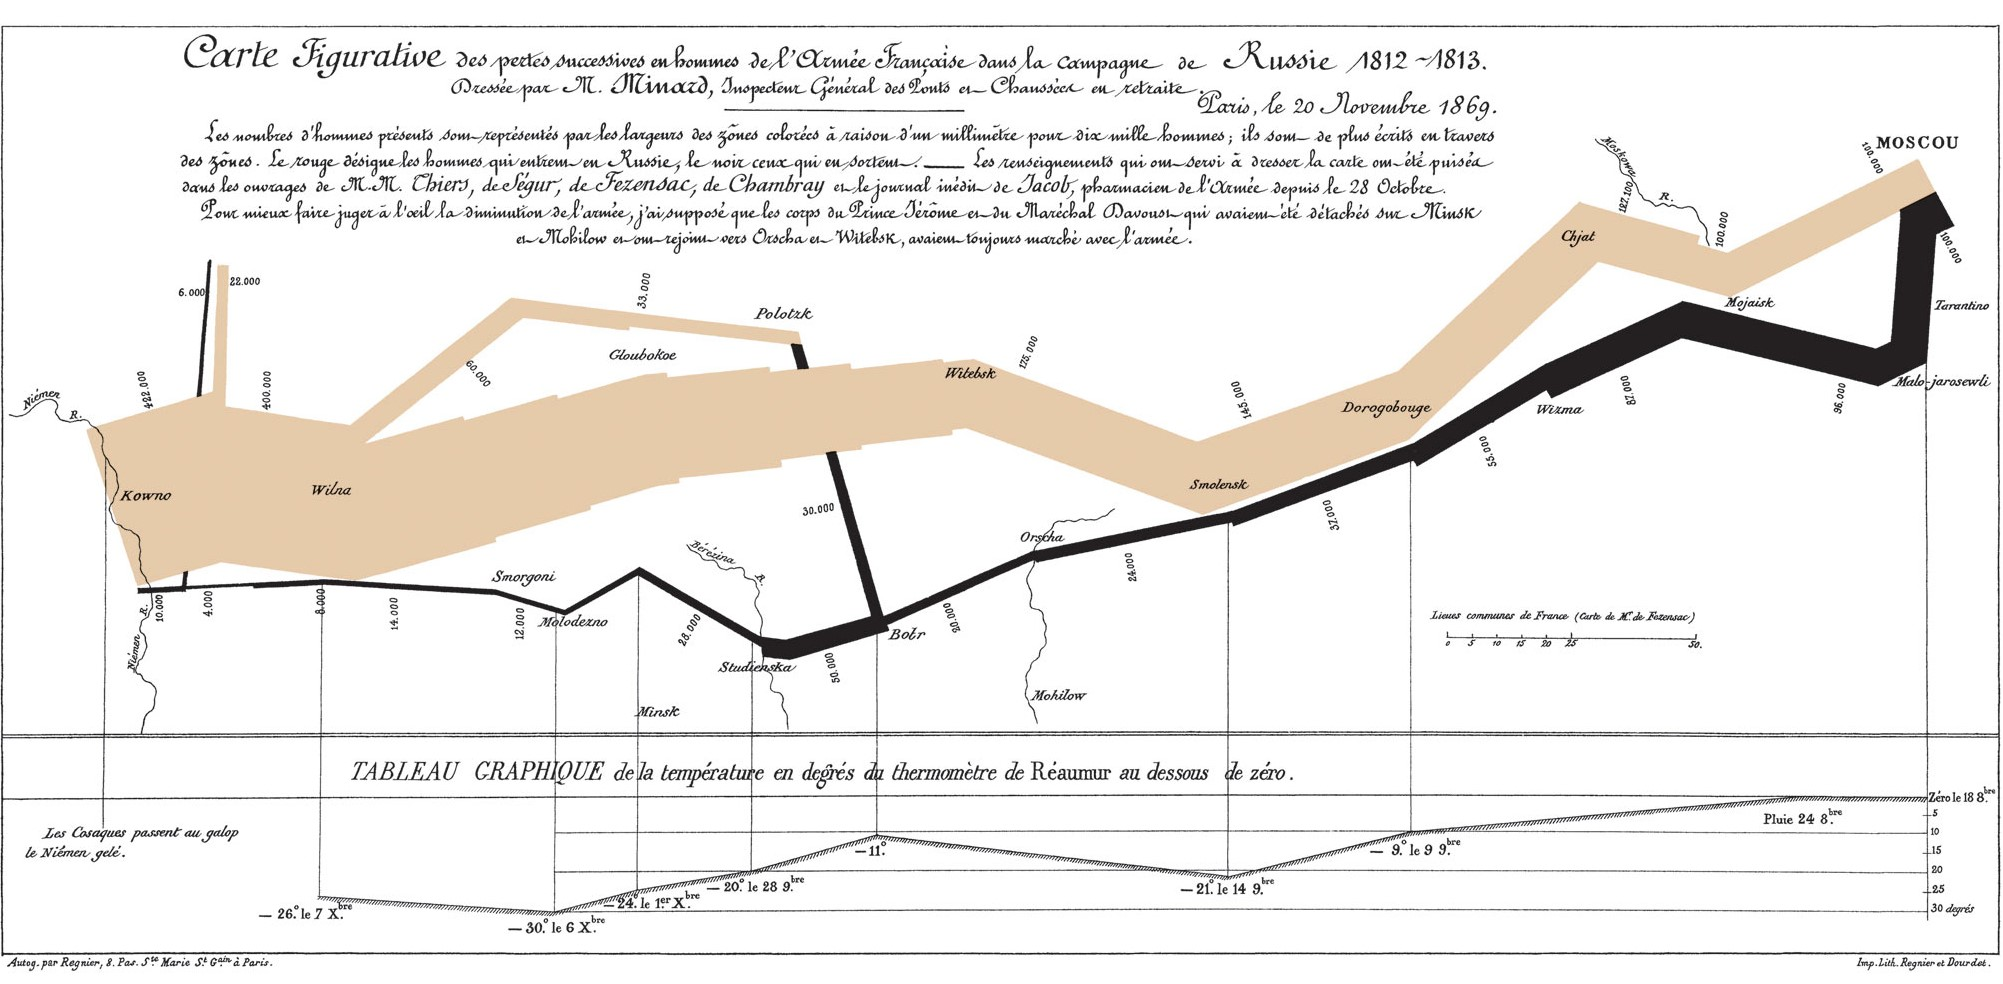
\includegraphics[width=0.8\linewidth]{figures/Minard.jpg}
    \par\end{centering}
    \caption[Napoleon's Invasion]{What may well be the greatest statistical graphic ever drawn~\cite{Tufte1983}\label{fig:MLP}}
\end{figure}

\section[More Lipsum]{Continuing on}\label{sec:lipsum}
\lipsum[6-10]~\cite{Min2023} \cref{fig:MLP}, \cref{tab:data}, \cref{eq:pn_taylor}, \cref{lst:listing-matlab}



\begin{table}[ht]
    \centering
    \small
    \begin{tabular}{SSSSSSSS} \toprule
        {\(m\)} & {\(\Re\{\underline{\mathfrak{X}}(m)\}\)} & {\(-\Im\{\underline{\mathfrak{X}}(m)\}\)} & {\(\mathfrak{X}(m)\)} & {\(\frac{\mathfrak{X}(m)}{23}\)} & {\(A_m\)} & {\(\varphi(m)\ /\ ^{\circ}\)} & {\(\varphi_m\ /\ ^{\circ}\)} \\ \midrule
        1  & 16.128 & +8.872 & 16.128 & 1.402 & 1.373 & -146.6 & -137.6 \\
        2  & 3.442  & -2.509 & 3.442  & 0.299 & 0.343 & 133.2  & 152.4  \\
        3  & 1.826  & -0.363 & 1.826  & 0.159 & 0.119 & 168.5  & -161.1 \\
        4  & 0.993  & -0.429 & 0.993  & 0.086 & 0.08  & 25.6   & 90     \\ \midrule
        5  & 1.29   & +0.099 & 1.29   & 0.112 & 0.097 & -175.6 & -114.7 \\
        6  & 0.483  & -0.183 & 0.483  & 0.042 & 0.063 & 22.3   & 122.5  \\
        7  & 0.766  & -0.475 & 0.766  & 0.067 & 0.039 & 141.6  & -122   \\
        8  & 0.624  & +0.365 & 0.624  & 0.054 & 0.04  & -35.7  & 90     \\ \midrule
        9  & 0.641  & -0.466 & 0.641  & 0.056 & 0.045 & 133.3  & -106.3 \\
        10 & 0.45   & +0.421 & 0.45   & 0.039 & 0.034 & -69.4  & 110.9  \\
        11 & 0.598  & -0.597 & 0.598  & 0.052 & 0.025 & 92.3   & -109.3 \\ \bottomrule
    \end{tabular}
    \caption[Random Data]{Table with random data.}\label{tab:data}
\end{table}

\begin{gather}
    V_{BE} = \frac{kT_0}{q} \Biggl\{ \ln{\biggl(\frac{I_C}{I_s T_0}\biggr)} + \Biggl[\ln{\biggl(\frac{I_C}{I_s T_0}\biggr)} - \biggl( \beta + \frac{E_{G_0}}{kT_0} \biggr) \Biggr] \biggl( \frac{T}{T_0} - 1 \biggr) \nonumber \\ - \frac{\beta}{2} {\biggl( \frac{T}{T_0} - 1 \biggr)}^2 + \cdots + \frac{\beta {(-1)}^{(n-1)}}{n(n-1)} {\biggl( \frac{T}{T_0} - 1 \biggr)}^n + \cdots \Biggr\}\label{eq:pn_taylor} \\
    V_{BE} > 4V_T,\qquad T < 2T_0 \nonumber
\end{gather}

\lstinputlisting[caption={[Matlab]Sample Code Listing Matlab}, label={lst:listing-matlab}, language=Matlab, style=Matlab-editor]{code/code_sample.m}
	
	% Bibliography file
	\bibliographystyle{bib/IEEEtranDOI} % custom style
	\makebibliography{bib/mybibliography}

	% Glossary
	\printglossary[type=main]

% End the document
\end{document} 